\documentclass[twocolumn]{article}
\usepackage{graphicx} % Required for inserting images
%\usepackage{subfig}
\usepackage{amsmath}
\usepackage{subcaption}
\usepackage[hyphens]{url}
\usepackage{hyperref}
\usepackage{tikz}
\usetikzlibrary{chains,shadows.blur}
\hypersetup{breaklinks=true}

\urlstyle{same}

\pagenumbering{gobble}
\title{\vspace{-1.25cm}Proof of Why Cat Toys End Up Under The Couch}
\author{Dave Pagurek}
\date{March 2026}

\begin{document}

\twocolumn[{
\vspace{-1.25cm}
\begin{center}
    \captionsetup{type=figure}
        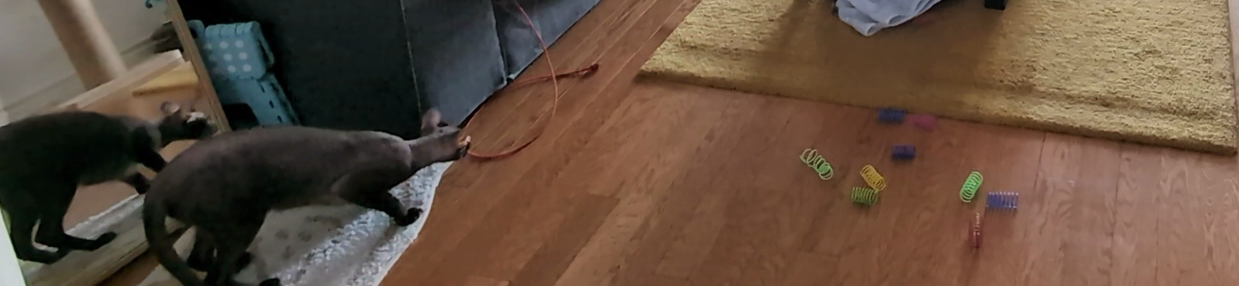
\includegraphics[width=\linewidth]{img/teaser.png}
    %\captionof{figure}{}
\end{center}
\maketitle
}]

\begin{abstract}
    When my cat's favourite toys are put out, they inevitably and rapidly end up shoved under the couch. This work confirms via computer simulation that cat toys will \emph{always} end up under the couch. When fitting the theoretical model to real-life observed speeds, we discovered the existence of \emph{dark car fur}, an unseen mass under the couch increasing the rate at which toys get stuck. The model predicts 10,000kg of dark cat fur under my couch to explain the motion of cat toys in my apartment. Since cats are perfect spheres and celestial bodies are perfect spheres, this model opens the door to a new understanding of  astrophysics.
\end{abstract}

\section{Introduction}

\begin{figure}
    \centering
    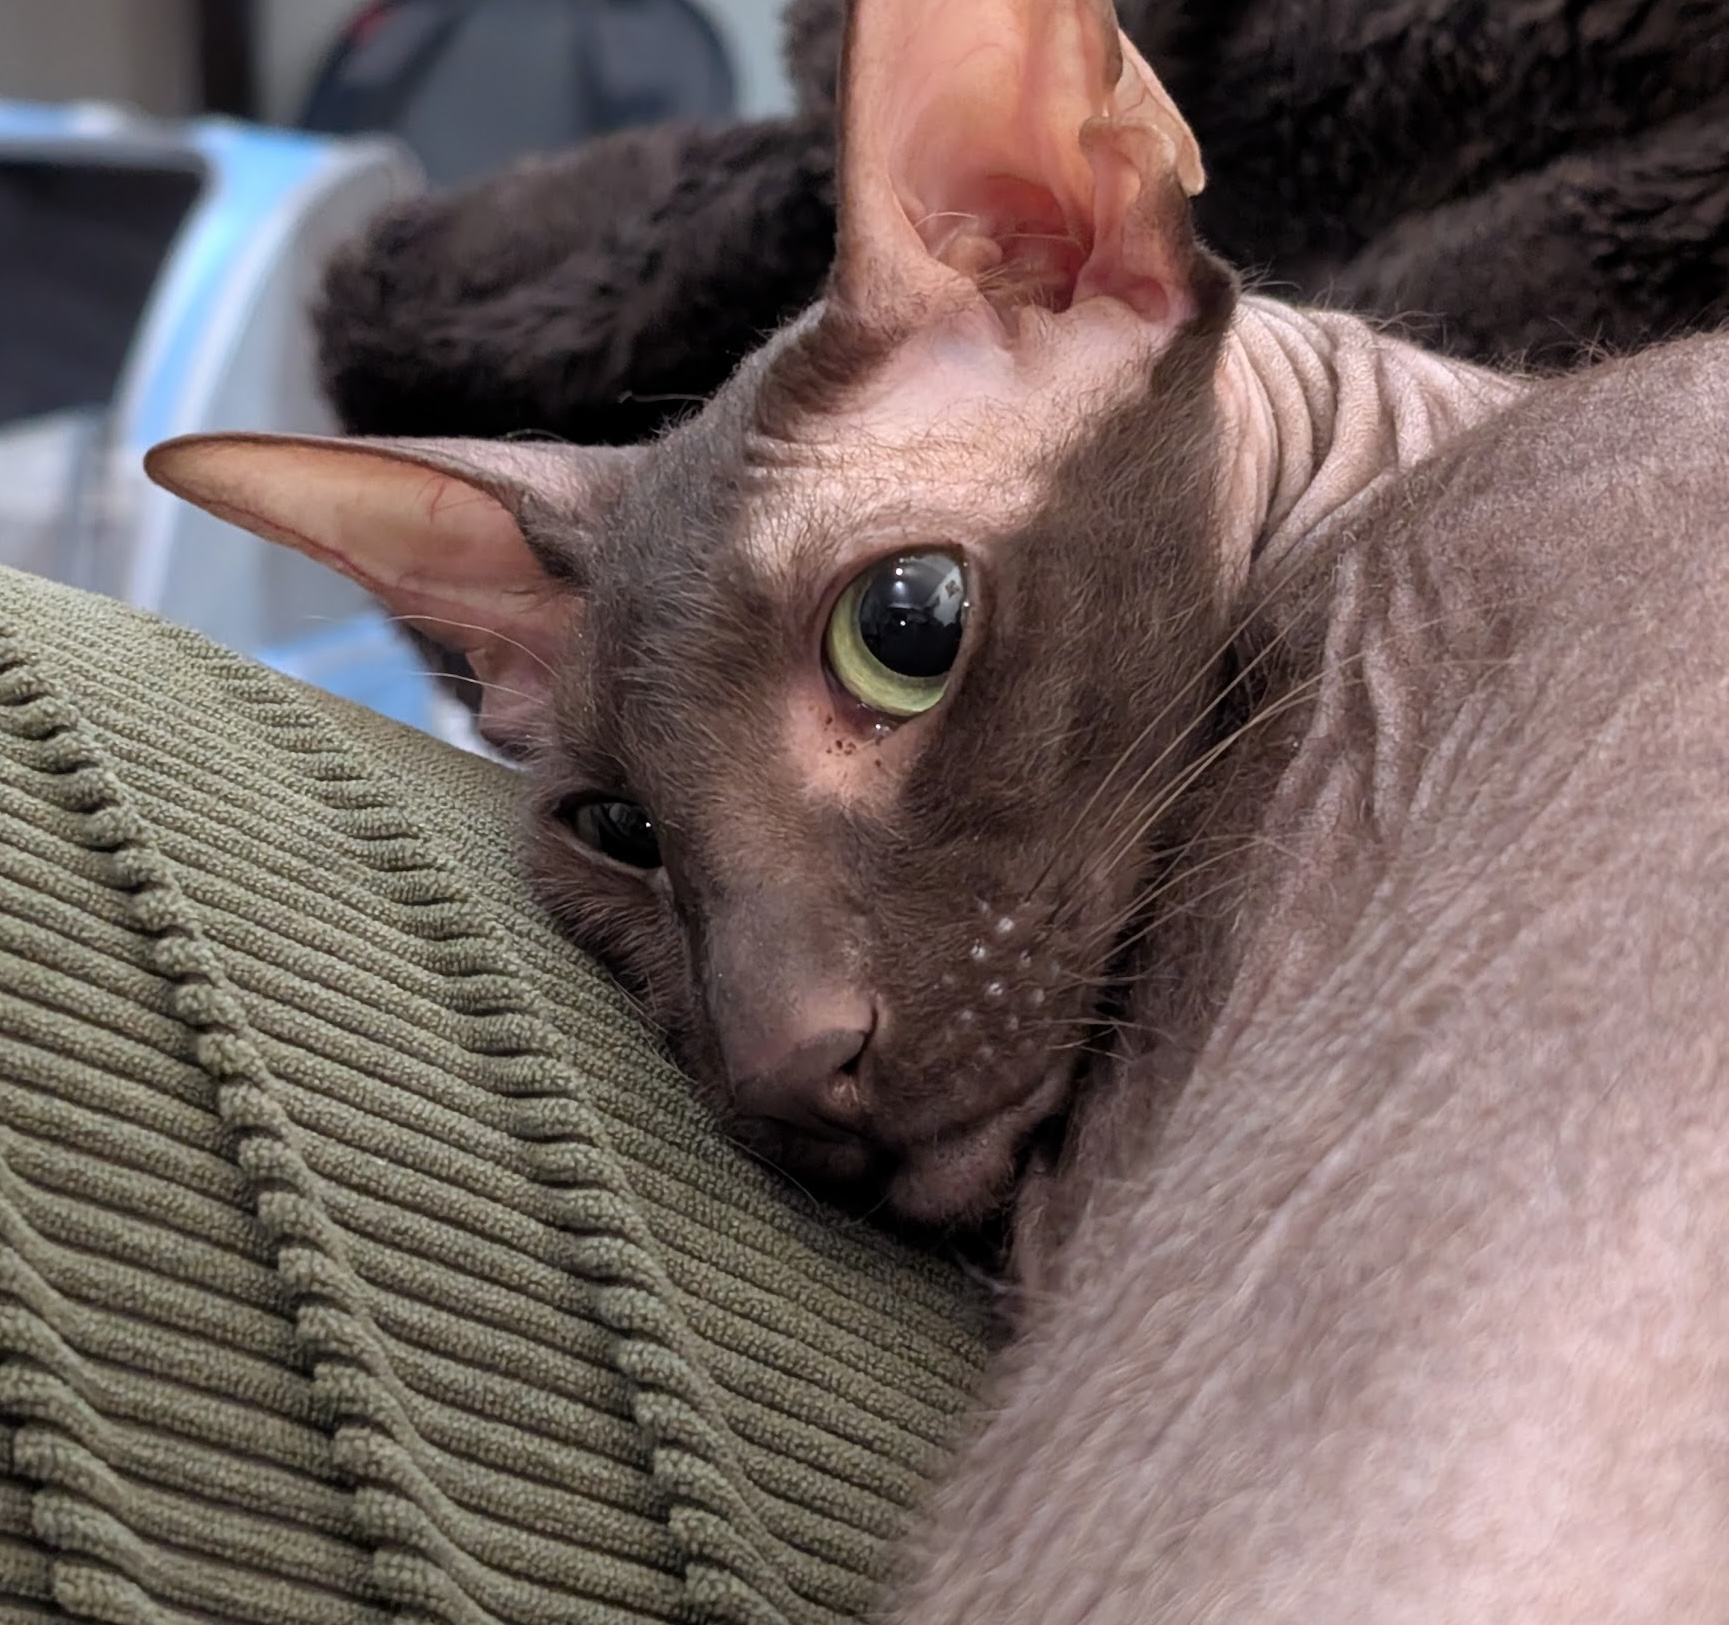
\includegraphics[width=0.68\linewidth]{img/perfect-sphere.jpg}
    \caption{My cat Pigeon, a perfect sphere.}
    \label{fig:cat}
\end{figure}

My cat Pigeon has a number of spring toys. They're quite a hit with her, as she can touch them and they skitter around the floor. However, they always end up under the couch again within fifteen minutes of being rescued out from under the couch. Is this an inevitability? How come it happens so quickly?

Current scientific modeling does not yet have an answer for these questions. This work proposes a probabilistic model of a cat playing with spring toys to determine whether or not this should be expected.


\section{Theoretical Model}

Without any loss of generality, we can assume each spring is an infinitesimally small point, and every cat is a perfect sphere.

In this model, our sphere cats can only push springs forward. They can do so from any side from which they can fit geometrically, with all possible angles having equal probability of being used. Each such push will happen over time according to a Poisson process, with an exponentially distributed random amount of time between pushes. The spring gets pushed a uniform random distance within a reasonable range. Springs reflect off of any surfaces.

We can effectively model my apartment as a 2D floor plan. While most objects interact with both the cat and the spring---the spring bounces off of them, and the cat cannot intersect with it while pushing the spring around---the couch is an area in which the spring is able to travel, but the cat cannot.

\section{Simulated results}

\begin{figure}
    \centering
    %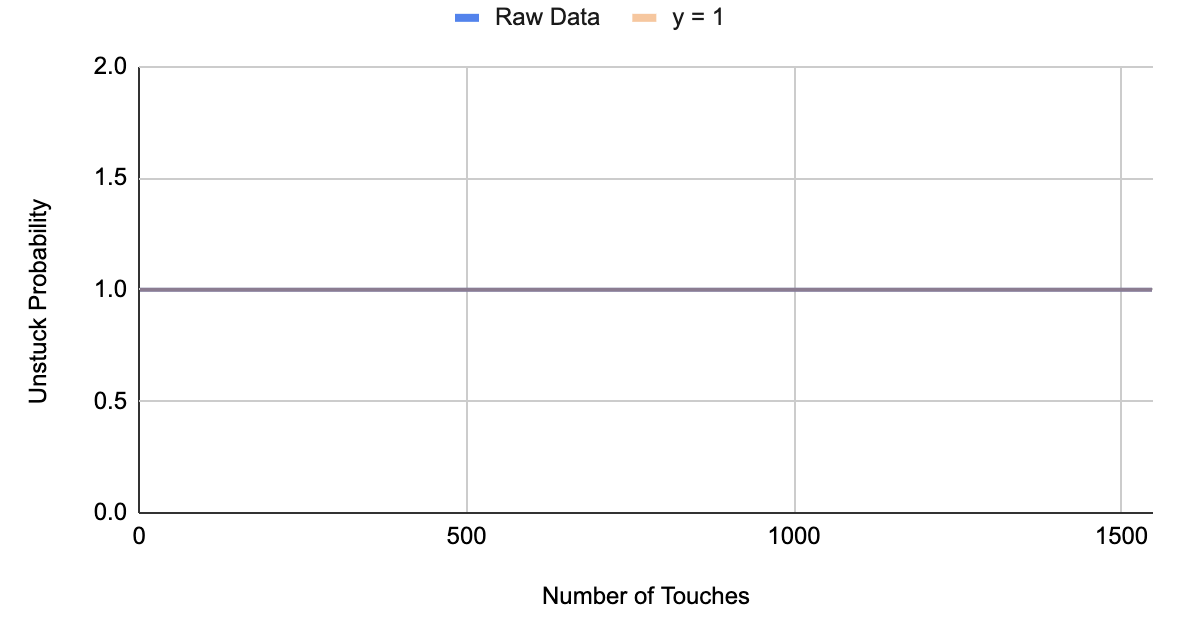
\includegraphics[width=0.78\linewidth]{img/no-couch.png}
    %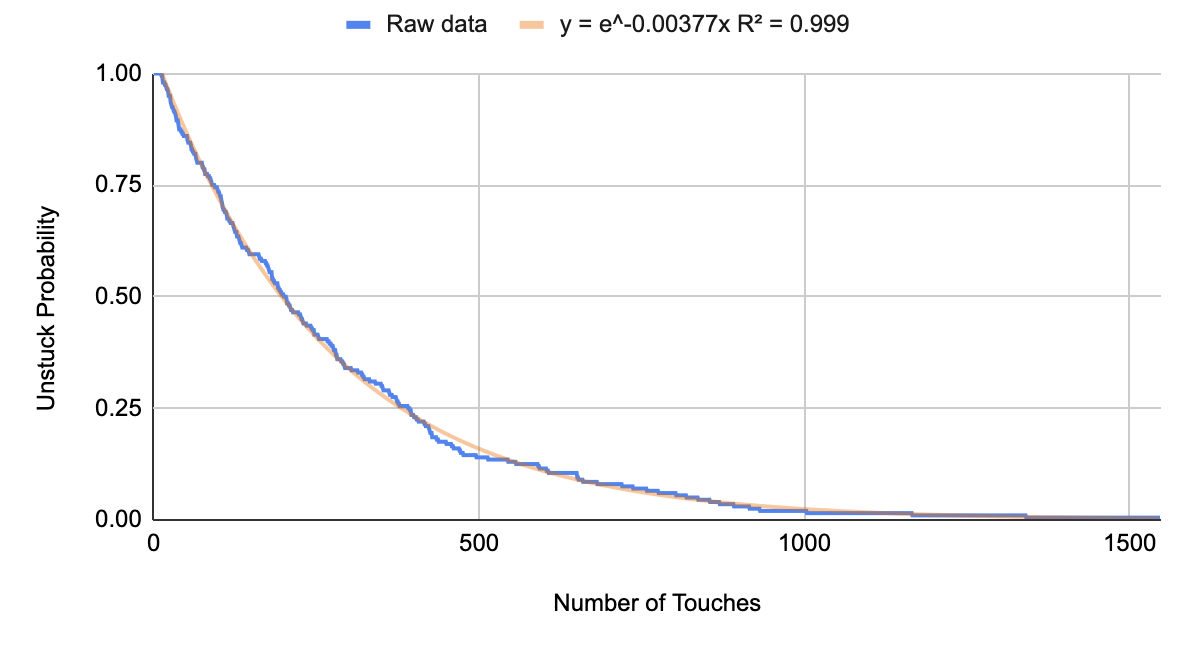
\includegraphics[width=0.78\linewidth]{img/loveseat.png}
    %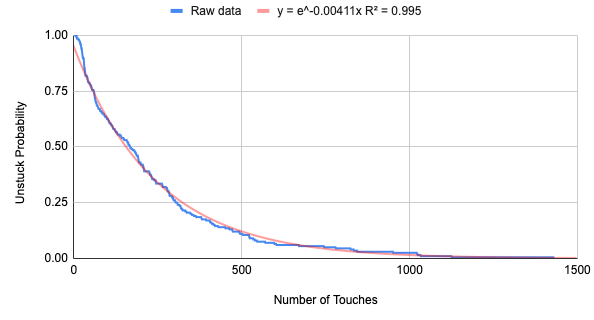
\includegraphics[width=0.78\linewidth]{img/couch.png}
    \begin{subfigure}[l]{0.48\textwidth} 
	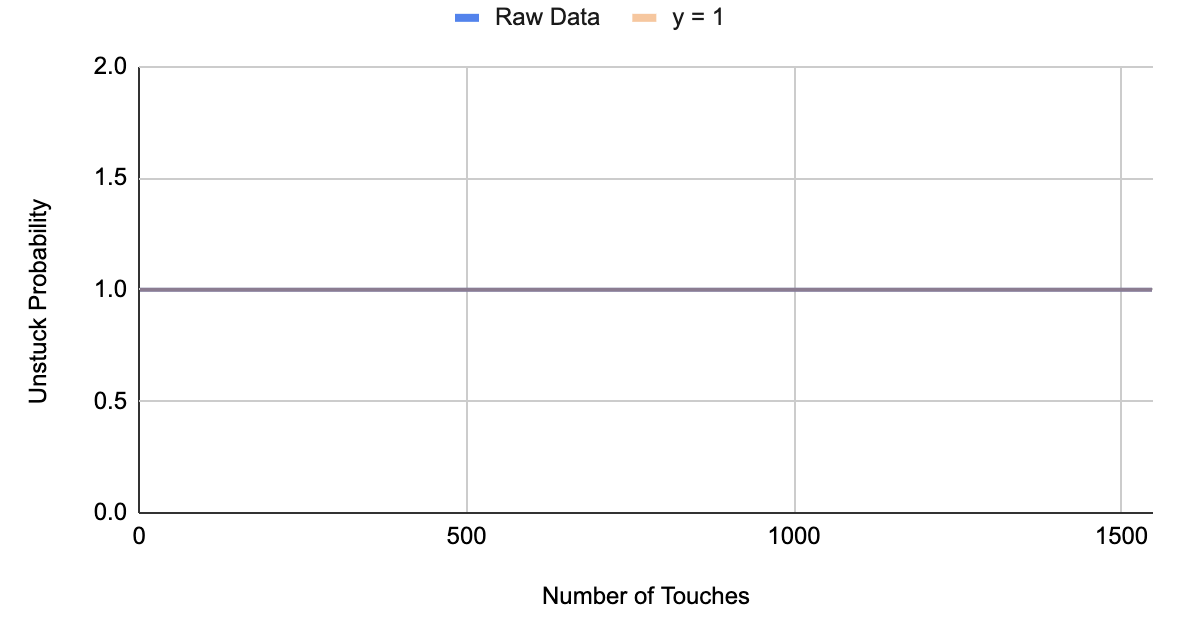
\includegraphics[width=\textwidth]{img/no-couch.png}
        	\caption{No couch} % Add subcaption text if desired, or use \subcaption* to suppress (a), (b), etc. labels
        	\label{fig:no-couch}
\end{subfigure}
\\[3ex]
\begin{subfigure}[l]{0.48\textwidth} 
	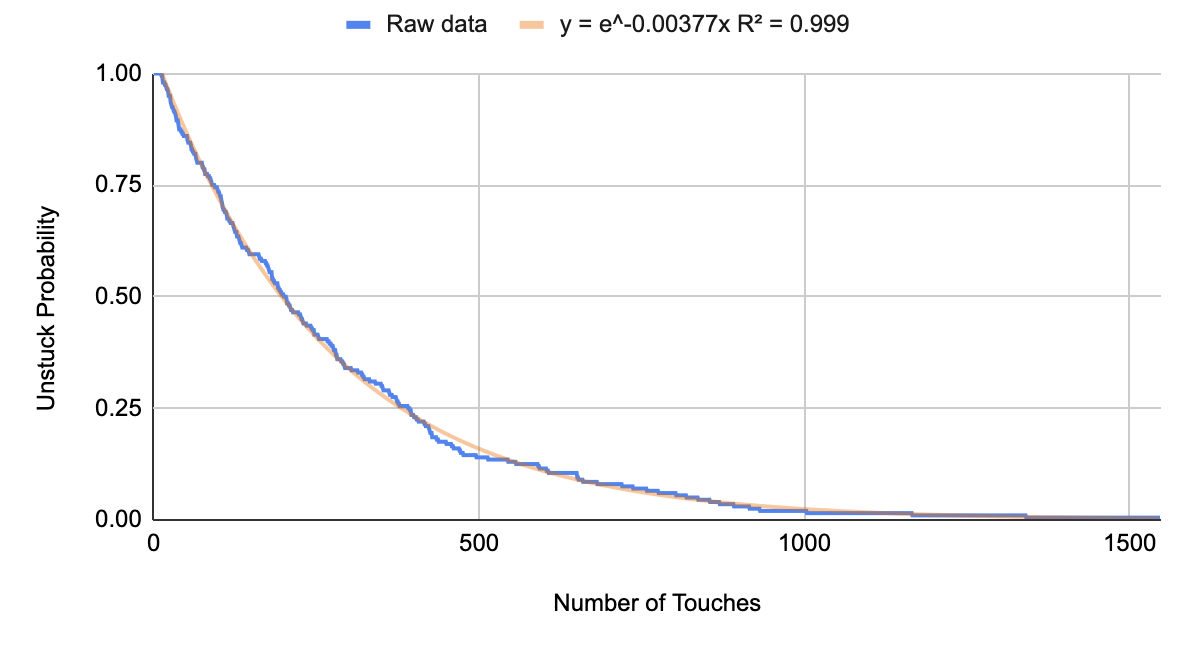
\includegraphics[width=\textwidth]{img/loveseat.png}
        	\caption{Loveseat (0.3\% of room area)} % Add subcaption text if desired, or use \subcaption* to suppress (a), (b), etc. labels
        	\label{fig:loveseat}
\end{subfigure}
\\[3ex]
\begin{subfigure}[l]{0.48\textwidth} 
	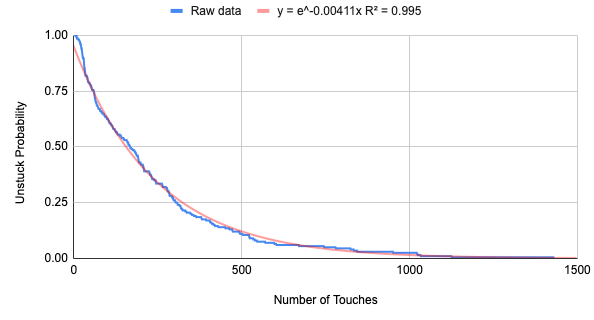
\includegraphics[width=\textwidth]{img/couch.png}
        	\caption{Couch (1.2\% of room area)} % Add subcaption text if desired, or use \subcaption* to suppress (a), (b), etc. labels
        	\label{fig:couch}
\end{subfigure}
    \caption{Probabilities of a spring being unstuck based on the number of touches from the cat.}
    \label{fig:probabilities}
\end{figure}


I simulated a few different setups 200 times each, recording after how many touches by the cat a spring ends up stuck somewhere, and graphed the probability that a spring will be under the couch after a given amount of touches. I tried this with an empty room, a room with a small loveseat, and a room with a wider couch. The graphed results are shown in Figure~\ref{fig:probabilities}. The horizontal axis is still in touches, not time, as experimental results are needed to find parameters for the Poisson distribution converting touches to time.

In Figure~\ref{fig:no-couch}, no couch is present. Springs never get stuck, even in corners of the room. Figure~\ref{fig:loveseat} introduces a small couch, and suddenly the springs start accumulating under it. The cumulative probability distribution of being unstuck follows an exponential distribution. Figure~\ref{fig:couch} uses a larger couch taking up more area of the room, and has similar results, but with the parameter $\lambda$ having greater magnitude, resulting in a steeper falloff.

This makes intuitive sense, in a monkeys-on-typewriters-producing-Shakespeare sort of way. If there is an area where a spring is able to get to that the cat cannot, and the spring effectively randomly traverses the space, then eventually, the spring will end up there. Once it ends up there, it gets stuck.

The question then is just why the springs end up under the couch \emph{so fast} in real life.

\section{Experimental Procedure}

I moved the couch out and rescued 12 springs that had accumulated under there. Afterwards, I set up a camera to track the activity of the test subject, my cat Pigeon, seen in Figure~\ref{fig:cat}. The 12 springs were dropped in a small pile in the middle of the room. Immediately, after six rapid spring touches, one spring ended up under the couch. Unfortunately, I then ran into a problem common in research in biology: the experimental subject, aware of the experiment, changed behavior. The subject noticed the camera and tripod, new items in the environment, and became self-conscious. Additionally, the novelty distracted from the springs.

There were enough moments without interruption that time between touches could be examined. Within these regions, wherein the test subject was ``locked in,'' I noted the times of touch events and created. Even when taken from discontinuous periods of being locked in, the times between events should still be samples of the same underlying exponential distribution, so these differences were counted up and placed into a histogram, shown in Figure~\ref{fig:touch-rate}.

\begin{figure}
    \centering
    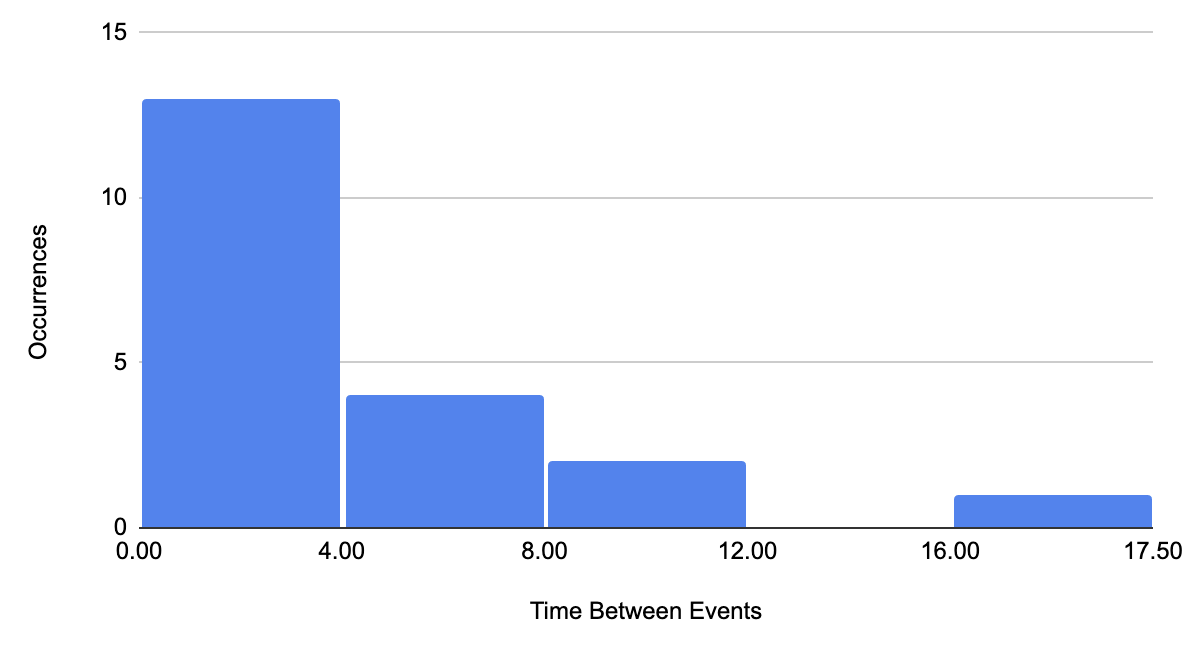
\includegraphics[width=\linewidth]{img/touch-rate.png}
    \caption{Histogram of the number of seconds between spring touches}
    \label{fig:touch-rate}
\end{figure}

Fitting an exponential distribution to the results in Figure~\ref{fig:touch-rate}, we get the parameter $\lambda=0.19$. The expected value of an exponential distribution is $\frac{1}{\lambda}$, which in this case gives us a 5.26 seconds between touches.

This value lets us convert touches in the simulation into time. For a single spring, we can use the fitted probability distribution in Figure~\ref{fig:couch} to determine that for the probability of a spring being under the couch to increase to 75\%, one needs to wait for 337 touches. At an average rate of 5.26 seconds between touches, this would take 29.5 minutes.

How do we square that with the fact that, when unobserved, springs disappear under the couch in 15 minutes? The probability of, say, 6 springs (in a smaller spring drop) all being under the couch in 15 minutes is $(e^{-0.00411 * 15*60/5.26})^6=1.4\%$!

\section{Dark Matter}

At this point it makes sense to take a cue from another area of physics in which we measured something different than our theory predicted: the expansion of our universe. Now, I'm not a physicist, but as a computer scientist, I feel qualified to confidently explain and conjecture in this area. The universe was expanding too fast, or slow, or something, than would be expected given its known mass. So that must mean that there's more bonus mass in there, dark matter, that we can't see. Clearly there is something similar going on with the couch.

I updated the simulation to include ``dark cat fur'': an invisible entity residing under the couch that directs springs towards it. In the simulation, it skews the angle a spring moves in to point closer towards the dark matter's center of mass proportional to the amount of dark matter and inversely proportional to the squared distance to it. We can then tweak the mass of the dark cat fur until we see the simulated springs disappear under the couch as quickly as we would expect to see in real life.

With $1 \cdot 10^4$kg of dark cat fur under the couch, there is an approximately 100\% probability that a spring is under the couch after 178 touches, which is expected to take 15.6 minutes.

\section{Conclusion}

Our experiments have definitively proven that you aren't imagining it: cat springs do in fact all end up under the couch. However, our best models predict that springs end up under the couch more slowly than we observe in real life. By introducing dark cat fur into the model, a cat spring equivalent of dark matter, the model is able to accurately predict real life results. This demonstrates that there is in fact tens of thousands of kilograms of cat spring material invisibly residing under our couches without us knowing.

These results open the door for new research in physics. Our current theory of dark matter, a stretch at best, is ripe for disruption. Since cats are perfect spheres, and most celestial bodies are perfect spheres, perhaps their motion is also affected by black cat fur. If there is so much black cat fur under our couches, just imagine how much black cat fur there must be out in the universe! I anticipate great leaps in our understanding of the universe in the near future thanks to the new ideas proposed in this work.

% \bibliographystyle{plainurl}
% \bibliography{main}

\end{document}
